\chapter{Introdu��o}
\label{cap:intro}

The goal of the present work is to study the Renshaw cells and its functions
using realistic computational models. Most of the data used here comes from
experiments carried out on the cat hindlimb. As cat experiments are seldom
performed nowadays, most of the recent data on the Renshaw cells come from 
rat. Therefore, rat data will be used with caution and expressly indicated.

\section{The motor system}
The \textbf{central nervous system} (CNS) comprises the brain and the
\textbf{spinal cord} (SC).
The latter is further subdivided into cervical, thoracic, lumbar, and sacral,
where each of these regions contains several segments.
The SC receives and processes information from muscles, joints, and skin and 
controls movement. In this context, the term \textbf{afferent} is used to
identify
the signals reaching the SC, whereas signals delivered to muscles are named
\textbf{efferent} \cite{kandel13}.

The type of muscle studied herein is the \textbf{skeletal muscle}, which
functions to move bones around joints, eyes within the head,
inhalation/exhalation, control facial expression, and speech \cite{bear16}.
Movements that decrease the angle between a segment and its proximal segment are
described as flexion, whereas movements that increase it are called extension
\cite{oxford}. Therefore, muscles can be classified as 
\textbf{flexors} and \textbf{extensors}. If muscles work together, they are
called
\textbf{synergists} of one another. If they pull a joint on the opposite
direction, they are called \textbf{antagonists} to one another \cite{bear16}.

Within each skeletal muscle there are hundreds of muscle fibers. They are
important not only for force generation, but also for \textbf{proprioception},
since the \textbf{muscle spindle}, which consists of several types of specialzed
skeletal muscle fibers contained in a fibrous capsule, provides feedback about
muscle length.

\section{The Spinal Cord Circuitry}
A cross section of the SC is shown in
Fig. \ref{fig:sc}. The central core is the
\textbf{gray matter}, which contains nerve cell bodies. The surrounding
\textbf{white matter}
accommodates ascending and descending axons.
The gray matter is further subdivided in \textbf{ventral} and
\textbf{dorsal horns}.

% TODO edit figure
\begin{figure}[ht!]
	\center
	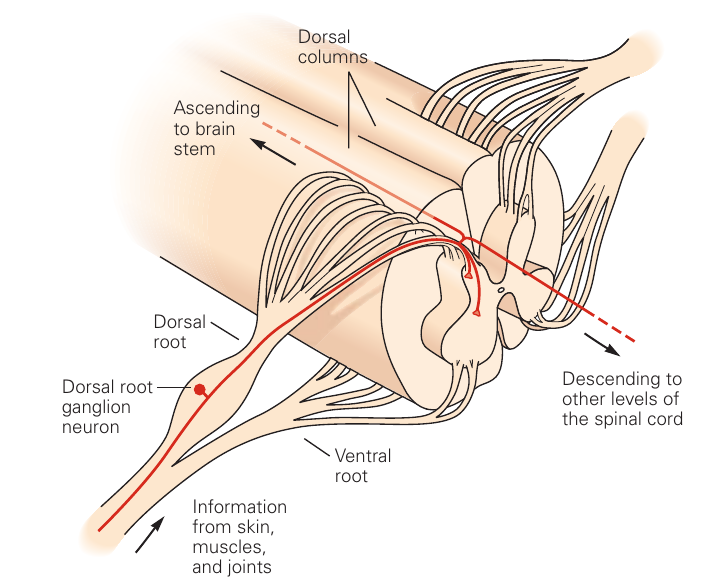
\includegraphics[scale=0.6]{sc.png}
	\caption{Cross section view of the spinal cord [Adapted from Kandel (2013)].}
	\label{fig:sc}
\end{figure}

The ventral
horn contains specialized types of neurons: the \textbf{motor neurons} (MNs),
which have \textbf{motor axons} innervating specific muscles, and the
\textbf{interneurons}
(INs), which
are involved in many neural circuits either at the segmental level or connecting 
with upper level neural structures.
The collection of one MN, its axon and all the muscle fibers it innervates is
called a \textbf{motor unit} (MN) \cite{liddell25,sherrington25}.

The dorsal root
consists of
afferent nerve fibers that carry information from muscles, tendons, joints and
the skin into the spinal cord,
whereas the ventral root, on the other hand, comprises axons innervating muscles
and muscle spindles.
There are two categories of MN: alpha ($\alpha$) and gamma ($\gamma$).The former
directly
initiates contractions of a muscle fibers. The collection of $\alpha$MNs that
innervate a single muscle is called a \textbf{motor nucleus} or \textbf{MN pool},
and motor nuclei form columns that run the length of the spinal cord
\cite{kandel13,bear16}.

The endings of motor axons innervating a muscle split into several fine branches
and form swellings called \textbf{synaptic boutons}, from which the MN releases
the neurotransmitter acetylcholine (ACh). Each bouton is positioned over a 
specialized region of the muscle membrane containing a high density of nicotic
type of ACh receptor. As a result, ACh released from motor axon terminals
interact with ACh receptors to produce an excitatory postsynaptic potential
(EPSP)\cite{kandel13}.

The $\alpha$MN are further subdivided into different types depending on the
properties of the neurons themselves and the muscle fibers they innervate:
fast, fatiguing (FF); fast, fatigue resistant (FR); and slow (S). % TODO ref and enoka obs and pool not homogeneous
% bear p 461, try to write it properly (fiber type and MU type)

% TODO anatomy figure of SC? (p 828)

\section{The Renshaw Cells}
The \textbf{Renshaw Cell} (RC) is an IN located at the ventral horn of the
spinal cord, medial to the motorneuronal columns. Its axon branchings spread over
distances
greater than 12mm rostrally or caudally \cite{jankowska71,jankowska73} and target a variety
of neurons.

The existence of the RC was first described in 1941 by Birdsey Renshaw
\cite{renshaw41} in an experiment in animals with the respective
dorsal root sectioned surgically, demonstrating that an
antidromic stimulation of motor axons caused an inhibition of
$\alpha$MNs
innervating the same (or \textbf{homonymous}) and synergistic muscles. Later, it was shown that this
inhibition is mediated through motor axon collaterals delivering excitatory synaptic inputs to
RCs, which in turn inhibit several MNs that innervate the respective muscle
\cite{eccles54}.

% TODO Figure with main connections and explaining

As one can see, this neural network contains a disynaptic pathway that starts
and ends at the same neuron: a MN provides an excitatory input to a RC, which in
turn provide inhibitory input to the homonymous MN. This spinal pathway provides
an inhibition known as \textbf{recurrent inhibition}. Other elements involved
on this scheme also receive this label, such as recurrent axon collaterals
and recurrent inhibitory postsynaptic potentials (IPSPs).

% TODO The connections shown is Figure ___ is a simplified view.

\subsection{Inputs to Renshaw Cells}
\subsubsection{From $\alpha$MNs}
Activation of RCs are obtained from stimulation of several nerves and smoothly
increase with increasing intensity of stimulation of individual nerves,
suggesting that a single RC is excited by axon collaterals of many MNs 
\cite{eccles54,eccles61b}. These
recurrent collaterals spread a distance of no more than 1 mm from their parent
cell body and have the majority of their synaptic boutons converging to
the area where the RCs are located \cite{cullheim78}. This caracteristic shows 
that excitation can be obtained only from motor nuclei located in the
neighbourhood of a given RC and is
therefore based on proximity factors. Furthermore, since some motor
nuclei can be as long as 10 mm, only part of a motor nucleus may project to a 
given RC \cite{romanes51,burke77}.

Besides proximity factors, converge to RCs are also based on functional factors.
This is supported by evidences showing that RCs are excited mainly by MNs 
of synergistic muscles and not by those of strict antagonists
\cite{ryall72,eccles61b}.

It should be noted that not all MNs give off recurrent collaterals.
Despite always being given off by MNs innervating ankle and knee muscles, they
are absent in MNs of short plantar foot muscles \cite{cullheim78}.

\subsubsection{From $\gamma$MNs}

\subsection{Outputs from Renshaw Cells}
% TODO distribution of IPSPs, here and later? There must be more to it
Recurrent inhibition is evoked in a number of motor nuclei after the stimulation
of the MNs of a given muscle. The recurrent IPSPs in the homonymous MNs are found
to be larger, but many other MNs are also strongly inhibitied
\cite{eccles54,eccles61b}.

% TODO RC functions

\section{Renshaw Cells Characteristics}

\section{ReMoto}
% TODO why exactly am I using a computational model here?
As shown previously, the RI circuit is considerably complex and is believed to
have important functions on the final output delivered to muscles. Despite all of
the efforts to comprehend the role of the RC on this network, 

% TODO there many other uses... maybe put the ones useful for me
On this aspect, a computational model can be very useful. It can be used to make
predictions, test theories or provide insights to experimentation. In the case of
the complex RI circuit, it might shed light over 



\index{problema}
O problema que esta tese aborda .... 

Algo importante a saber ao escrever em portugu�s � que os arquivos .tex devem ser salvos com decodifica��o ISO 8859-15.

\section{Objetivos}
\index{objetivos}
\index{exemplo! sigla}
O objetivo central do trabalho apresentado, realizado na \ac{USP} (este foi um exemplo de uso de sigla),  � ...


\section{Estrutura do texto}

\index{estrutura}
Este texto est� organizado da seguinte maneira ... 



